\documentclass[conference]{IEEEtran}
\usepackage[utf8]{inputenc}
\usepackage[italian]{babel}
\usepackage{graphicx}
\usepackage{cite}
\usepackage{amsmath}
\usepackage{booktabs}
\usepackage{float}
\usepackage{url}

\title{Storage Chiave-Valore Replicato e Consistente in Go}

\author{
\IEEEauthorblockN{Federico Cola}
\IEEEauthorblockA{
Corso di Sistemi Distribuiti e Cloud Computing\\
Universit\`a degli Studi di Roma ``Tor Vergata''\\
Email: federicola00@gmail.com}
}

\begin{document}

\maketitle

\begin{abstract}
Questo lavoro presenta un key-value store distribuito, replicato e
fortemente consistente, costruito in Go attorno a un'implementazione da
zero dell'algoritmo di consenso Raft. Il sistema è composto da tre
tipologie di nodo — consensus node stateful, client proxy stateless e
servizio di snapshot \& backup stateless — che comunicano esclusivamente
via gRPC e Protocol Buffers, e integra due pattern architetturali, Service
Discovery e Circuit Breaker, per la scoperta dinamica del leader e
l'isolamento dei nodi non raggiungibili. Il deployment è containerizzato
con Docker Compose e verificato su una vera istanza AWS EC2. Il sistema è
stato valutato con due esperimenti: scalabilità (tempo di risposta delle
RPC al variare del numero di nodi, da 3 a 20) e fault-tolerance (tempo di
rielezione e convergenza dopo il crash del leader). I risultati sono
coerenti con la teoria di Raft — latenza di lettura indipendente dal
numero di nodi, latenza di scrittura che cresce solo con quorum di
maggioranza numerosi, tempi di rielezione in linea con i timeout
configurati — e il percorso sperimentale ha messo in luce l'importanza di
un ambiente di misura isolato per benchmark di latenza affidabili.
\end{abstract}

\section{Introduction}

Questo lavoro presenta la progettazione e l'implementazione di un
key-value store distribuito, replicato e fortemente consistente,
sviluppato nell'ambito del progetto B5 del corso di Sistemi Distribuiti e
Cloud Computing. Il sistema non si appoggia a nessun database centrale:
la consistenza dello stato tra le repliche è garantita interamente
dall'algoritmo di consenso distribuito \textbf{Raft}~\cite{ongaro2014raft},
implementato da zero.

L'architettura è composta da tre tipologie di nodo con responsabilità
distinte: un cluster di \emph{consensus node} stateful, che eseguono
l'algoritmo di consenso e mantengono lo stato replicato; un
\emph{client proxy} stateless, che instrada le richieste dei client verso
il nodo Leader corrente scoprendolo dinamicamente; e un servizio di
\emph{snapshot e backup} stateless, che effettua periodicamente il
checkpoint dello stato applicativo. La comunicazione interna tra i nodi
avviene tramite RPC su gRPC e Protocol Buffers, e il sistema integra due
pattern architetturali — Service Discovery e Circuit Breaker — per
gestire rispettivamente la scoperta dinamica del Leader e l'isolamento
dei nodi non raggiungibili. Il deployment è containerizzato con Docker
Compose ed è stato verificato su un'istanza reale AWS EC2.

Lo sviluppo è stato affiancato dall'uso di strumenti di intelligenza
artificiale, impiegati principalmente come supporto alla scrittura delle
sezioni di codice, mentre le scelte progettuali, la verifica del
comportamento del sistema e l'interpretazione dei risultati sperimentali
sono state guidate direttamente dall'autore. L'intero percorso di lavoro è
tracciato attraverso un sistema di versionamento (Git/GitHub), con commit
incrementali e descrittivi per ciascuna fase; il codice sorgente completo
e commentato è disponibile pubblicamente all'indirizzo
\url{https://github.com/Cellu83/sdcc-Progetto-b5-kvstor}.

Il resto del report è organizzato come segue: la Sezione~\ref{sec:background}
richiama i concetti di consenso distribuito necessari a comprendere le
scelte progettuali; la Sezione~\ref{sec:design} descrive l'architettura
del sistema; la Sezione~\ref{sec:details} entra nel merito delle scelte
implementative più significative; la Sezione~\ref{sec:results} presenta
i risultati sperimentali di scalabilità e fault-tolerance; la
Sezione~\ref{sec:discussion} discute tali risultati e i limiti noti del
sistema; la Sezione~\ref{sec:conclusions} chiude il lavoro.

\section{Background}
\label{sec:background}

In un sistema distribuito che replica il proprio stato su più nodi per
tollerare guasti, il problema centrale è far sì che tutte le repliche
concordino sulla stessa sequenza di operazioni, anche in presenza di
crash di singoli nodi o di ritardi di rete. Risolvere questo problema
senza un coordinatore centrale (che sarebbe esso stesso un singolo punto
di fallimento) è l'obiettivo degli algoritmi di \emph{consenso
distribuito}.

Tra le soluzioni note, Paxos~\cite{lamport2001paxos} è storicamente la più
citata, ma è notoriamente difficile da adattare e da implementare
correttamente. Per questo progetto si è scelto
\textbf{Raft}~\cite{ongaro2014raft}, progettato esplicitamente per essere
semplice senza sacrificare le garanzie di correttezza di Paxos,
scomponendo il problema in tre sotto-problemi relativamente indipendenti:
elezione del leader, replicazione del log e sicurezza.

I concetti chiave di Raft rilevanti per le sezioni successive sono:

\begin{itemize}
  \item \textbf{Term}: un contatore logico monotono crescente che
  identifica un intervallo di tempo con al più un Leader. Ogni messaggio
  tra nodi porta il term del mittente, e un term più recente prevale
  sempre su uno più vecchio.
  \item \textbf{Ruoli}: ogni nodo è in un dato momento Follower,
  Candidate o Leader. Un Follower che non riceve heartbeat dal Leader
  diventa, entro un timeout randomizzato, un Candidate e avvia una nuova
  elezione; vince chi ottiene il voto della maggioranza dei nodi.
  \item \textbf{Log replication}: solo il Leader accetta scritture dai
  client; le aggiunge al proprio log e le replica ai Follower. Un'entry è
  \emph{committata}, e quindi applicabile alla state machine, solo dopo
  essere stata replicata su una maggioranza dei nodi.
  \item \textbf{Election restriction}: un candidato può ottenere un voto
  solo se il proprio log è aggiornato almeno quanto quello di chi vota —
  condizione che impedisce di eleggere un Leader che perderebbe entry già
  committate.
  \item \textbf{La regola di sicurezza \S5.4.2}: un leader può committare per semplice conteggio di maggioranza solo le entry del proprio term corrente, mai quelle di un term precedente (anche se già su una maggioranza); deve aspettare che si comitti insieme a (almeno) un'entry del proprio term corrente. È una regola sottile ma essenziale per la correttezza, discussa più avanti (Sezioni~\ref{sec:details} e~\ref{sec:discussion}) anche alla luce di un'osservazione empirica avvenuta durante il deployment su cloud.
\end{itemize}

Infine, la comunicazione tra i nodi richiede un meccanismo di RPC
efficiente e tipizzato: il sistema usa gRPC con interfacce definite in
Protocol Buffers, sia per le RPC interne dell'algoritmo di consenso
(\texttt{RequestVote}, \texttt{AppendEntries}) sia per l'API applicativa
esposta ai client (\texttt{Get}/\texttt{Put}/\texttt{Delete}).

\section{Solution Design}
\label{sec:design}

Il sistema è composto da tre tipologie di nodo, ciascuna un binario Go
indipendente, che comunicano esclusivamente via RPC gRPC/Protocol Buffers
(Figura~\ref{fig:architecture}).

\begin{figure}[t]
\centering
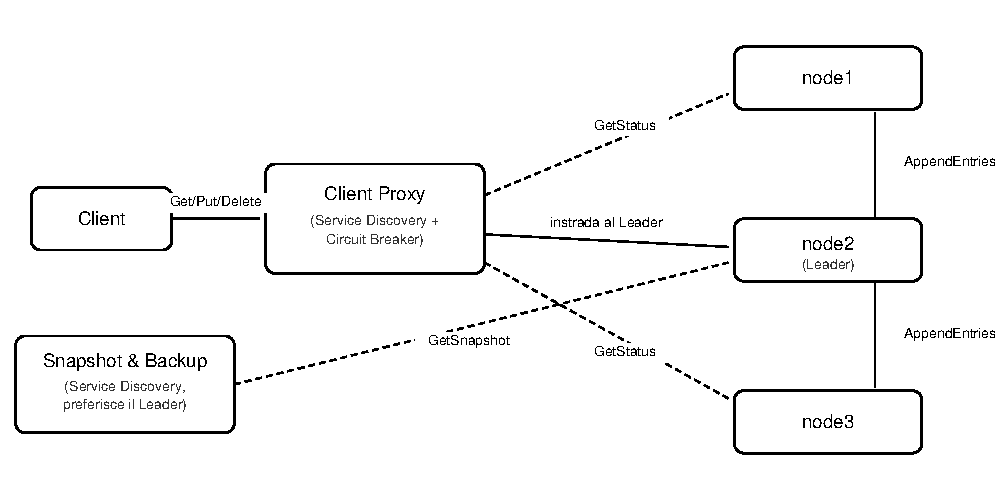
\includegraphics[width=\columnwidth]{architecture.pdf}
\caption{Architettura del sistema: tre tipologie di nodo comunicanti via
gRPC. Frecce continue: RPC applicative/di replica. Frecce tratteggiate:
RPC di sola lettura usate per la Service Discovery e per lo Snapshot \&
Backup service.}
\label{fig:architecture}
\end{figure}

\textbf{Consensus node} (stateful): eseguono l'algoritmo Raft e mantengono
lo stato replicato — sia il log persistito (\texttt{CurrentTerm},
\texttt{VotedFor}, le entry) sia la state machine chiave-valore in
memoria. Espongono \texttt{RaftService} (\texttt{RequestVote},
\texttt{AppendEntries}, e le RPC di sola lettura \texttt{GetStatus} e
\texttt{GetSnapshot}) e, solo se correntemente Leader, rispondono anche
alle richieste applicative di \texttt{KVStoreService}.

\textbf{Client proxy} (stateless): unico punto di contatto per i client
esterni. Non mantiene stato applicativo proprio; il suo unico compito è
instradare in modo trasparente ogni richiesta verso il Leader corrente,
riprovando verso un altro nodo se quello contattato non lo è (più), realizza questo tramite i due pattern architetturali
richiesti dalla traccia.

\textbf{Snapshot \& backup service} (stateless): interroga periodicamente
un consensus node raggiungibile per ottenere un'istantanea dello stato
applicativo corrente, e la scrive su un checkpoint esterno persistente —
un backup indipendente dal ciclo di vita di ogni singolo
nodo.

\subsection{Service Discovery}

Nessun componente del sistema conosce, staticamente, l'indirizzo
dell'attuale Leader — perché può cambiare in qualunque momento, per
elezione o per crash. Il pattern Service Discovery
(\texttt{internal/discovery}) risolve questo interrogando periodicamente i
nodi noti tramite la RPC di sola lettura \texttt{GetStatus}, che
restituisce chi il nodo interrogato ritiene sia il Leader corrente. Sia il
Client proxy sia lo Snapshot \& backup service riusano lo stesso
meccanismo: partono da una lista statica di nodi seed (nota da
configurazione) e mantengono da lì in poi una vista sempre aggiornata di
peer e Leader, senza mai avere un indirizzo fisso scritto nel codice.

\subsection{Circuit Breaker}

Il Circuit Breaker (\texttt{internal/proxy}) applicato dal Client
proxy a ogni indirizzo tiene traccia dei fallimenti consecutivi verso
quell'indirizzo con tre stati: \emph{closed} (funzionamento normale),
\emph{open} (troppi fallimenti consecutivi: le chiamate verso quell'indirizzo
vengono scartate immediatamente, senza nemmeno provare la rete, per un
periodo di raffreddamento), \emph{half-open} (raffreddamento scaduto: una
sola chiamata di prova per verificare se il nodo è tornato disponibile).
Combinato con la Service Discovery, questo permette al proxy di isolare
rapidamente un nodo caduto e ridirigersi verso il Leader corrente senza
pagare ripetutamente il costo dei timeout di rete verso nodi che sa già
irraggiungibili.

\section{Solution Details}
\label{sec:details}

\subsection{Configurazione esterna, nessun valore hard-coded}

All'interno del progetto nessun parametro operativo (ID del nodo,
indirizzi dei peer, porte, timeout di elezione, intervallo di heartbeat,
livello di log) vive nel codice: tutto passa da un file YAML caricato
tramite struct tipizzate (\texttt{internal/config}), che vengono validate al momento del caricamento. Questa scelta, fa in modo che in Docker Compose si possano semplicemente passare configurazioni diverse
(Sezione~\ref{sec:docker}), e che lo strumento usato per generare i cluster di
N nodi per gli esperimenti di scalabilità (Sezione~\ref{sec:results}) riusi
direttamente le stesse struct invece di modificare il file YAML manualmente.

\subsection{Persistenza atomica su disco}

I tre pezzi di stato che Raft impone di rendere durevoli —
\texttt{CurrentTerm}, \texttt{VotedFor}, e il log delle entry — sono
scritti su disco (\texttt{internal/raftlog}) con uno schema di scrittura
atomica: prima su un file temporaneo, poi con una \texttt{rename} sopra il
file definitivo. Questo garantisce che un crash del processo a metà
scrittura non lasci mai uno stato corrotto o parziale: al riavvio il nodo
trova o lo stato precedente (se il crash è avvenuto prima della rename) o
quello nuovo completo (se dopo), mai una via di mezzo. Lo stesso schema è
riusato, senza modifiche concettuali, dal servizio Snapshot per scrivere i
propri checkpoint esterni.

Da notare, e rilevante per i risultati della Sezione~\ref{sec:results}:
\texttt{commitIndex} e \texttt{lastApplied} sono deliberatamente
\emph{volatili} e si azzerano a ogni riavvio del
processo: è così che il paper di Raft li definisce, e
il sistema si comporta correttamente anche in questo caso limite grazie
alla regola di sicurezza \S5.4.2 (Sezione~\ref{sec:background}).

\subsection{Replicazione del log: \texttt{nextIndex} e \texttt{matchIndex}}

Per ogni follower, il Leader mantiene due valori volatili che si ricostruiscono da zero a ogni nuova elezione, \texttt{nextIndex[id]} e
\texttt{matchIndex[id]}, rispettivamente il prossimo indice di log da
inviare a quel follower e l'indice più alto che si sa già replicato su di
lui.

La replica verso ogni peer è innescata sia periodicamente, a ogni tick
dell'heartbeat (50ms), sia immediatamente dopo una \texttt{Propose}, così
una nuova scrittura non deve attendere il prossimo tick per iniziare a
essere replicata. Per ciascun follower il Leader invia, in una singola RPC
\texttt{AppendEntries}, \texttt{PrevLogIndex}/\texttt{PrevLogTerm} (il
punto del log da cui il follower dovrebbe già essere allineato) seguiti da
\emph{tutte} le entry dal proprio \texttt{nextIndex} fino alla fine del
log — non una entry alla volta.

L'aggiornamento di \texttt{nextIndex}/\texttt{matchIndex} avviene in modo
sincrono, non appena arriva la risposta a quella RPC:

\begin{itemize}
  \item se il follower accetta (\texttt{Success = true}, perché la sua
  entry a \texttt{PrevLogIndex} coincide con quella del Leader),
  \texttt{matchIndex[id]} viene alzato all'indice più alto appena
  confermato — con una guardia che ne impedisce la retrocessione, dato che
  più chiamate verso lo stesso follower possono essere in volo
  contemporaneamente (una dal ciclo di heartbeat, una da una
  \texttt{Propose}) e le risposte possono arrivare in un ordine diverso da
  come sono partite. L'avanzamento di \texttt{matchIndex} innesca subito,
  nella stessa sezione critica, il tentativo di far avanzare il
  \texttt{commitIndex} del cluster controllando la maggiornata dei nodi (Sezione~\ref{sec:background}).
  \item se il follower rifiuta (\texttt{Success = false}, conflitto di log
  a \texttt{PrevLogIndex}), \texttt{nextIndex[id]} viene decrementato di
  uno, e si riproverà al giro successivo con un punto di partenza più
  indietro.
\end{itemize}

Un dettaglio rilevante per la velocità di recupero di un follower rimasto
indietro: il passo indietro (\texttt{nextIndex--}) avviene una posizione
alla volta finché non si trova il punto d'accordo col Leader, ma una volta
trovato, il passo in avanti recupera \emph{tutto} il ritardo accumulato in
un'unica RPC (tutte le entry mancanti insieme), non un'entry per round.

\subsection{Backoff di riconnessione gRPC vs. timeout di elezione}
\label{sec:backoff}

Testando dal vivo scenari di crash e riavvio ripetuti (uccidendo e
riavviando nodi in varie combinazioni tramite Docker), è emerso un pattern
sistematico: un nodo riavviato avviava \emph{sempre} una nuova elezione,
non riconosceva mai in silenzio il Leader già attivo — anche quando
rientrava in poche centinaia di millisecondi. La causa non era casuale ma
strutturale: \texttt{internal/raft/client.go} riusa la stessa connessione
gRPC verso ogni peer (\texttt{Client.connFor}), ed è corretto farlo per
evitare di riaprire una connessione TCP a ogni RPC. Il problema è che gRPC,
di default, applica un backoff di riconnessione con \texttt{BaseDelay} di
1 secondo — pensato per reti geografiche reali — quando una connessione
cade. Quando un nodo veniva ucciso e poi riavviato, il Leader restava
fermo nel proprio timer di backoff (\textgreater{}1s) prima di ritentare
la connessione verso di lui, ben oltre il timeout di elezione del nodo
riavviato (150--300ms): quest'ultimo scadeva sempre prima di ricevere un
heartbeat, e si candidava — spesso vincendo, dato che il suo log restava
comunque aggiornato quanto quello degli altri.

Corretto impostando un \texttt{BaseDelay} molto più breve (50ms) tramite
\texttt{grpc.WithConnectParams} su ogni connessione verso i peer. Verificato
con un test locale con processi nativi: un follower ucciso e riavviato
torna a riconoscere il Leader esistente in meno di 150ms, senza elezione.
Ripetendo la stessa prova in container Docker, il comportamento è invece
risultato variabile — a volte il nodo riconosce il Leader, a volte si
candida comunque. Il motivo non è più il backoff (ormai trascurabile), ma
un limite fisico diverso: il tempo che Docker impiega a far ripartire
davvero il container (processo, listener gRPC) prima che il Leader possa
riconnettersi, che può da solo superare il timeout di elezione a seconda
del carico della macchina — un vincolo della piattaforma di
containerizzazione, non del codice applicativo.

\subsection{Compattazione dello storico in checkpoint esterni}

Il servizio Snapshot \& backup soddisfa il requisito di "scaricare e
compattare i log storici in file di checkpoint stabili": la RPC
\texttt{GetSnapshot} non restituisce il log grezzo, ma lo stato corrente
della state machine (\texttt{Store.Snapshot()}) — l'intera storia di
operazioni \texttt{Put}/\texttt{Delete} già compattata nel suo risultato
finale. Il servizio scarica questo stato e lo scrive su un checkpoint
esterno persistente, in sola lettura verso i nodi, indipendente dal ciclo
di vita di ognuno di essi.

Un'implementazione più tradizionale di Raft userebbe tipicamente lo
snapshot anche per comprimere il log sui consensus node stessi (troncando
le entry già incluse nello snapshot). In questo progetto si è scelto
deliberatamente di \emph{non} farlo: il servizio resta puramente esterno,
senza mai modificare il log o gli indici di nessun consensus node. La
motivazione è non rimettere in discussione la matematica degli indici
(\texttt{commitIndex}, \texttt{matchIndex}, la regola \S5.4.2) già
verificata e mantenere il servizio funzionante maggiormente separato dal sistema del cluster.
\subsection{Containerizzazione}
\label{sec:docker}

Il deployment usa un solo Dockerfile generico multi-stadio, parametrizzato
via build-arg (\texttt{SERVICE}), invece di tre Dockerfile quasi identici:
uno stadio di build con l'intero toolchain Go, e uno stadio finale
minimale che contiene solo il binario compilato. \texttt{docker-compose.yml}
definisce 7 servizi (5 consensus node, proxy, snapshot) che riferiscono
tutti lo stesso Dockerfile con un \texttt{SERVICE} diverso; le
configurazioni per l'ambiente Docker sono identiche a quelle locali tranne
per gli indirizzi dei peer, che usano i nomi dei servizi Compose invece di
\texttt{localhost} (risolti via il DNS interno della rete bridge di
Compose). Containerizzare non ha richiesto nessuna modifica al codice
applicativo — conseguenza diretta della configurazione esterna descritta
sopra.

Il deployment è stato verificato su una vera istanza AWS EC2
(\texttt{t2.micro}, AWS Academy Learner Lab), non solo in locale
(Figura~\ref{fig:ec2-evidence}): i 5 container avviati con
\texttt{docker compose up -d}, l'elezione del leader osservata nei log del
container stesso (con i peer risolti via DNS come \texttt{node1:50051}, non
\texttt{localhost}), l'istanza raggiungibile dall'esterno sul suo IP
pubblico, e la porta del proxy (50060) aperta nel Security Group per
consentire chiamate reali da fuori l'istanza.

\begin{figure*}[t]
\centering
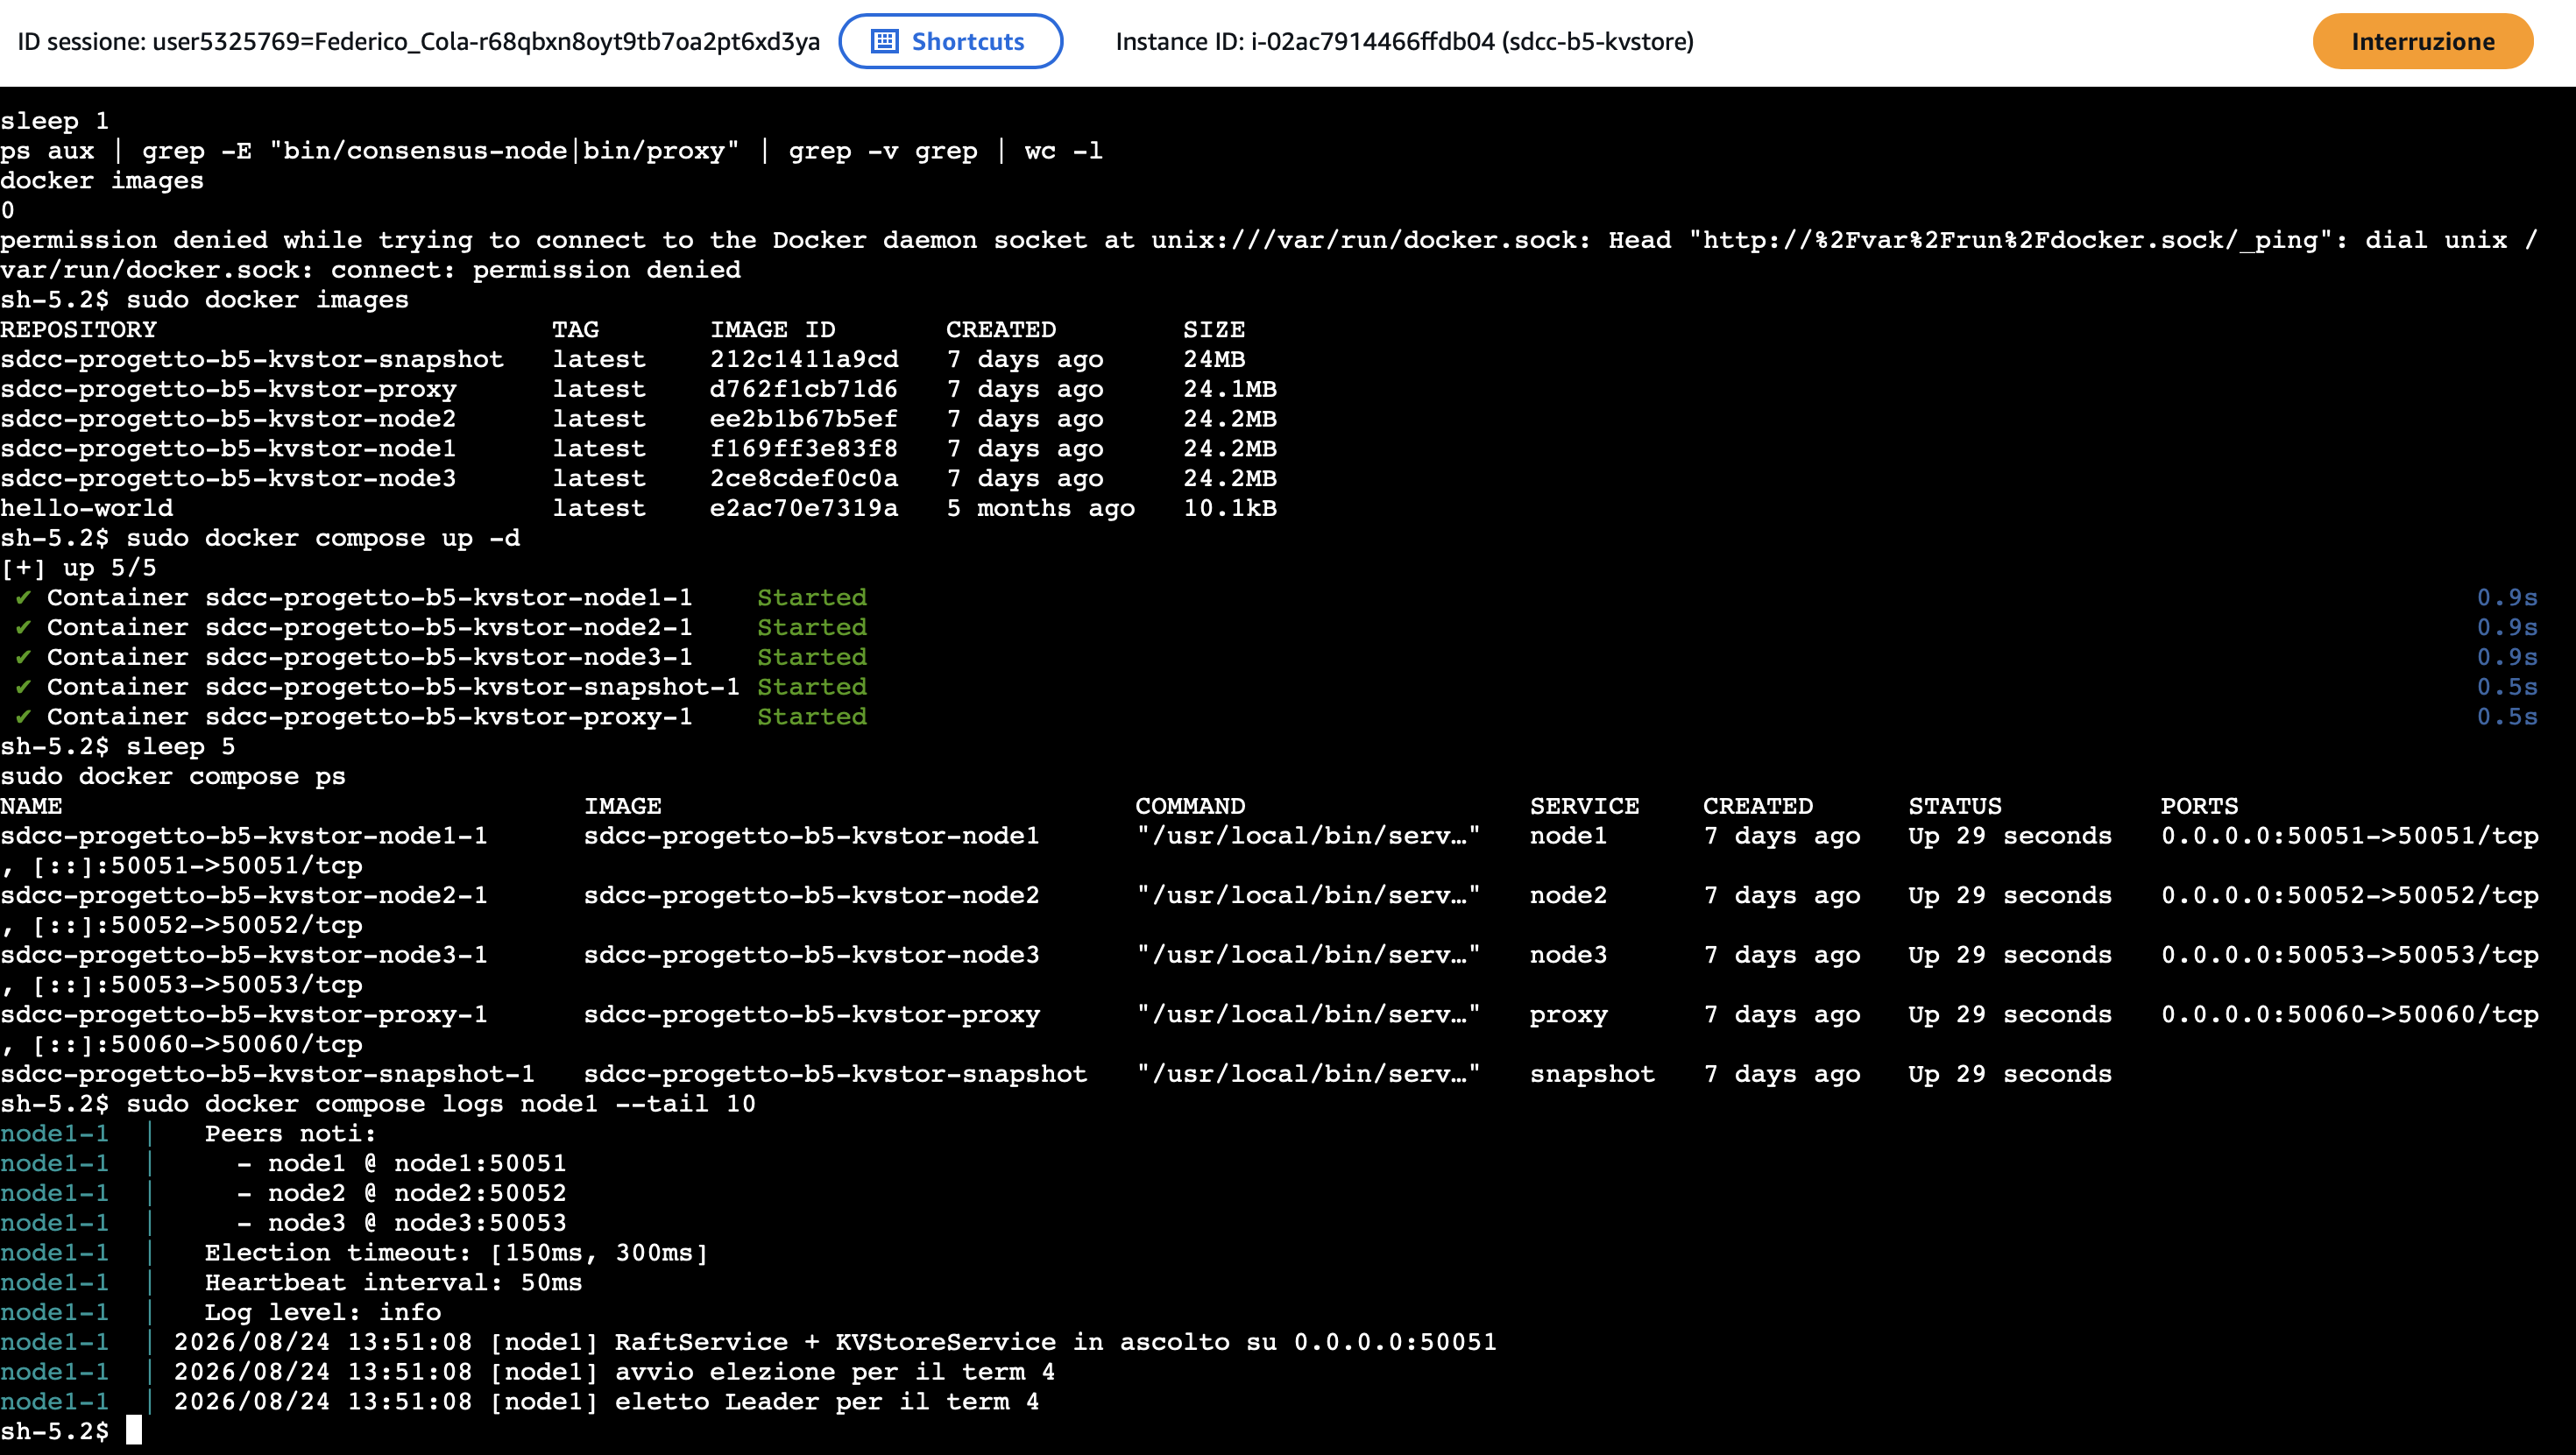
\includegraphics[width=0.92\textwidth]{docker-terminal.png}\\[4pt]
\begin{minipage}{0.47\textwidth}
\centering
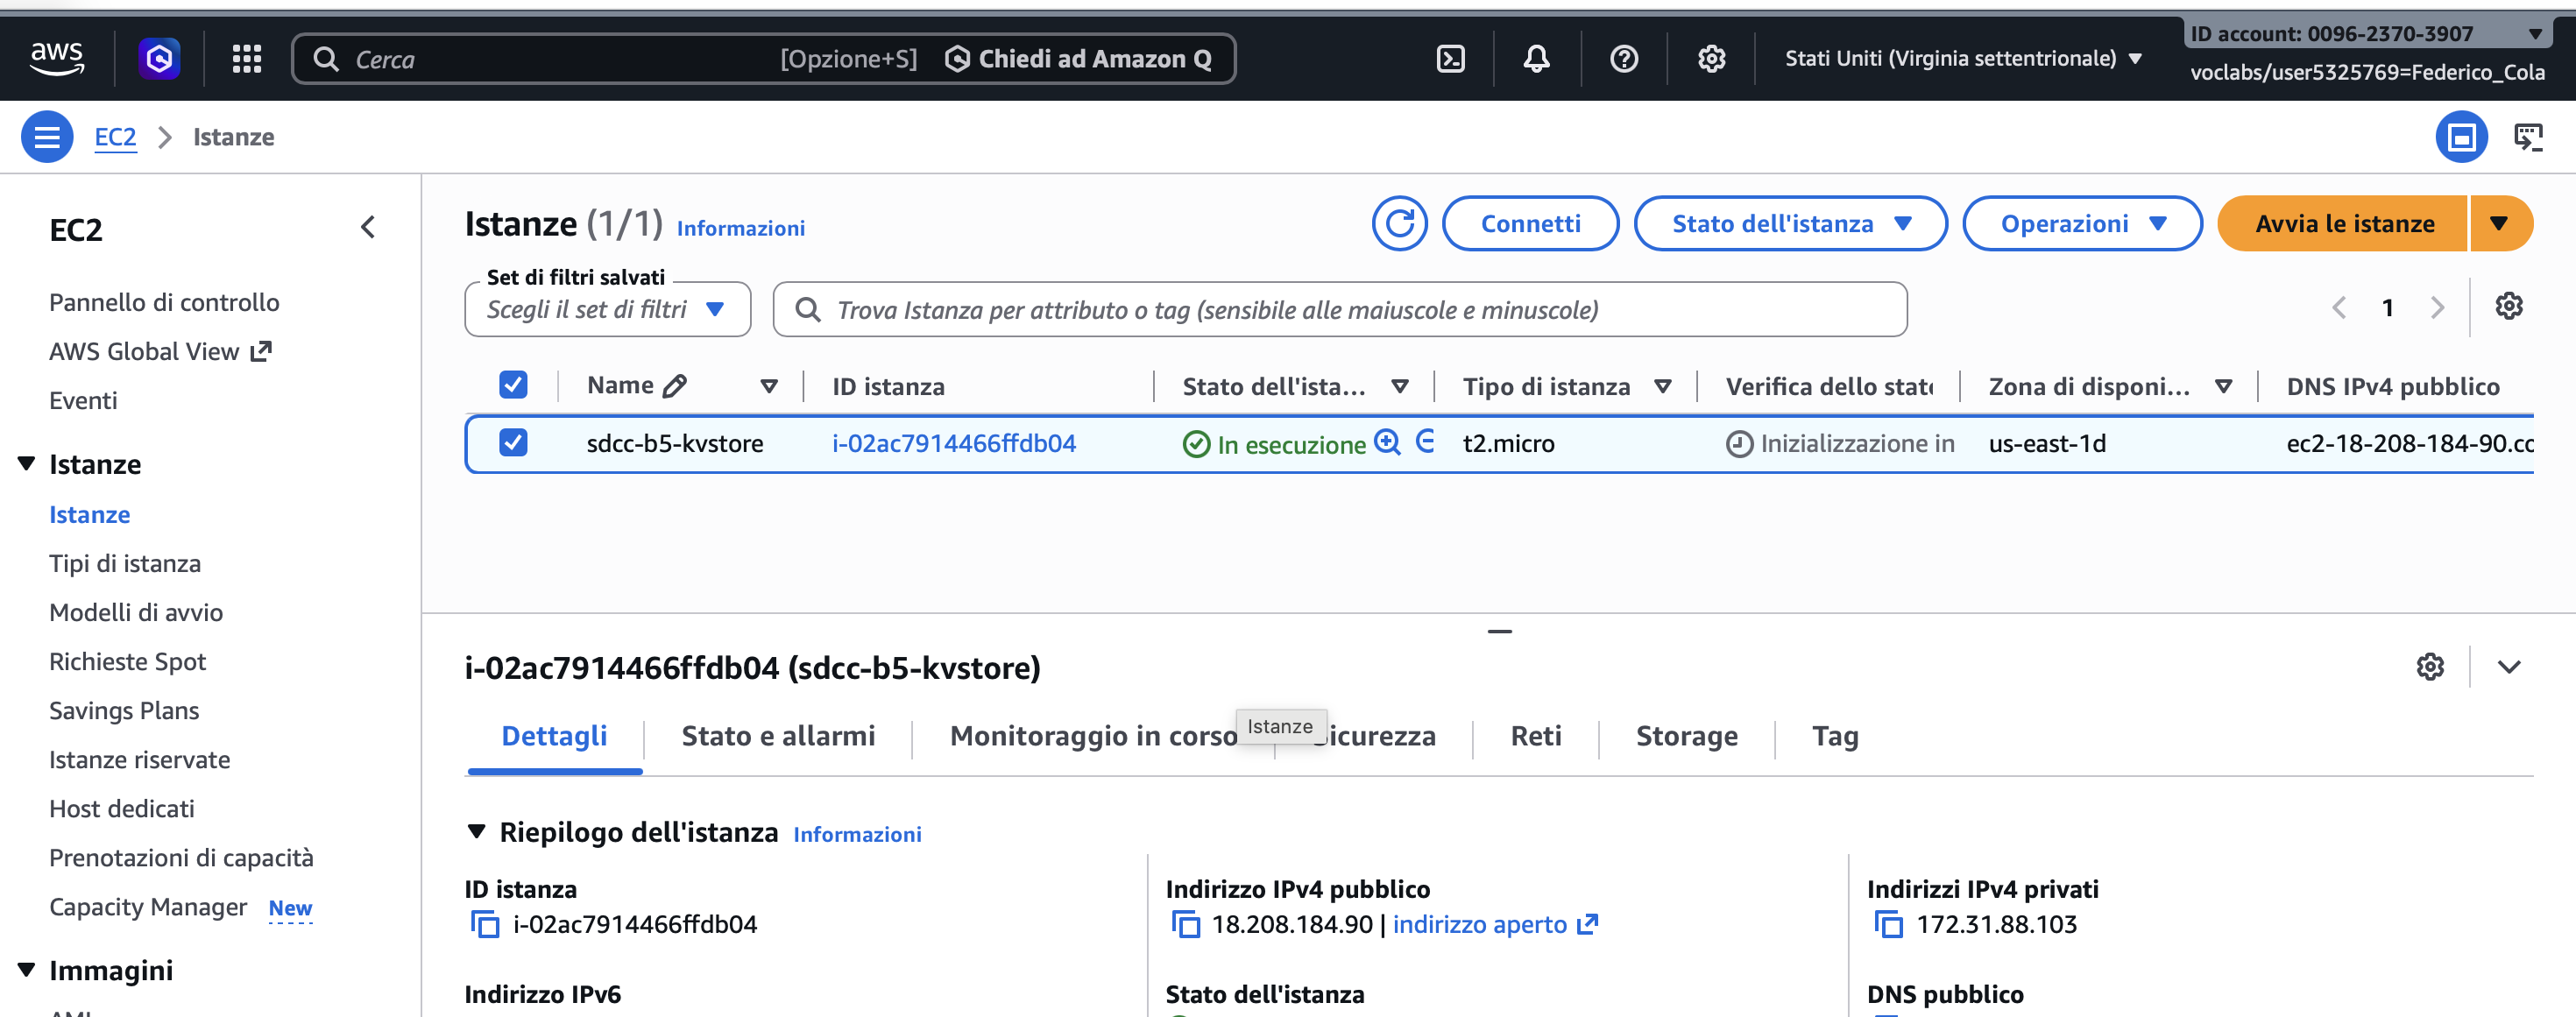
\includegraphics[width=\textwidth]{ec2-instance.png}
\end{minipage}
\hfill
\begin{minipage}{0.47\textwidth}
\centering
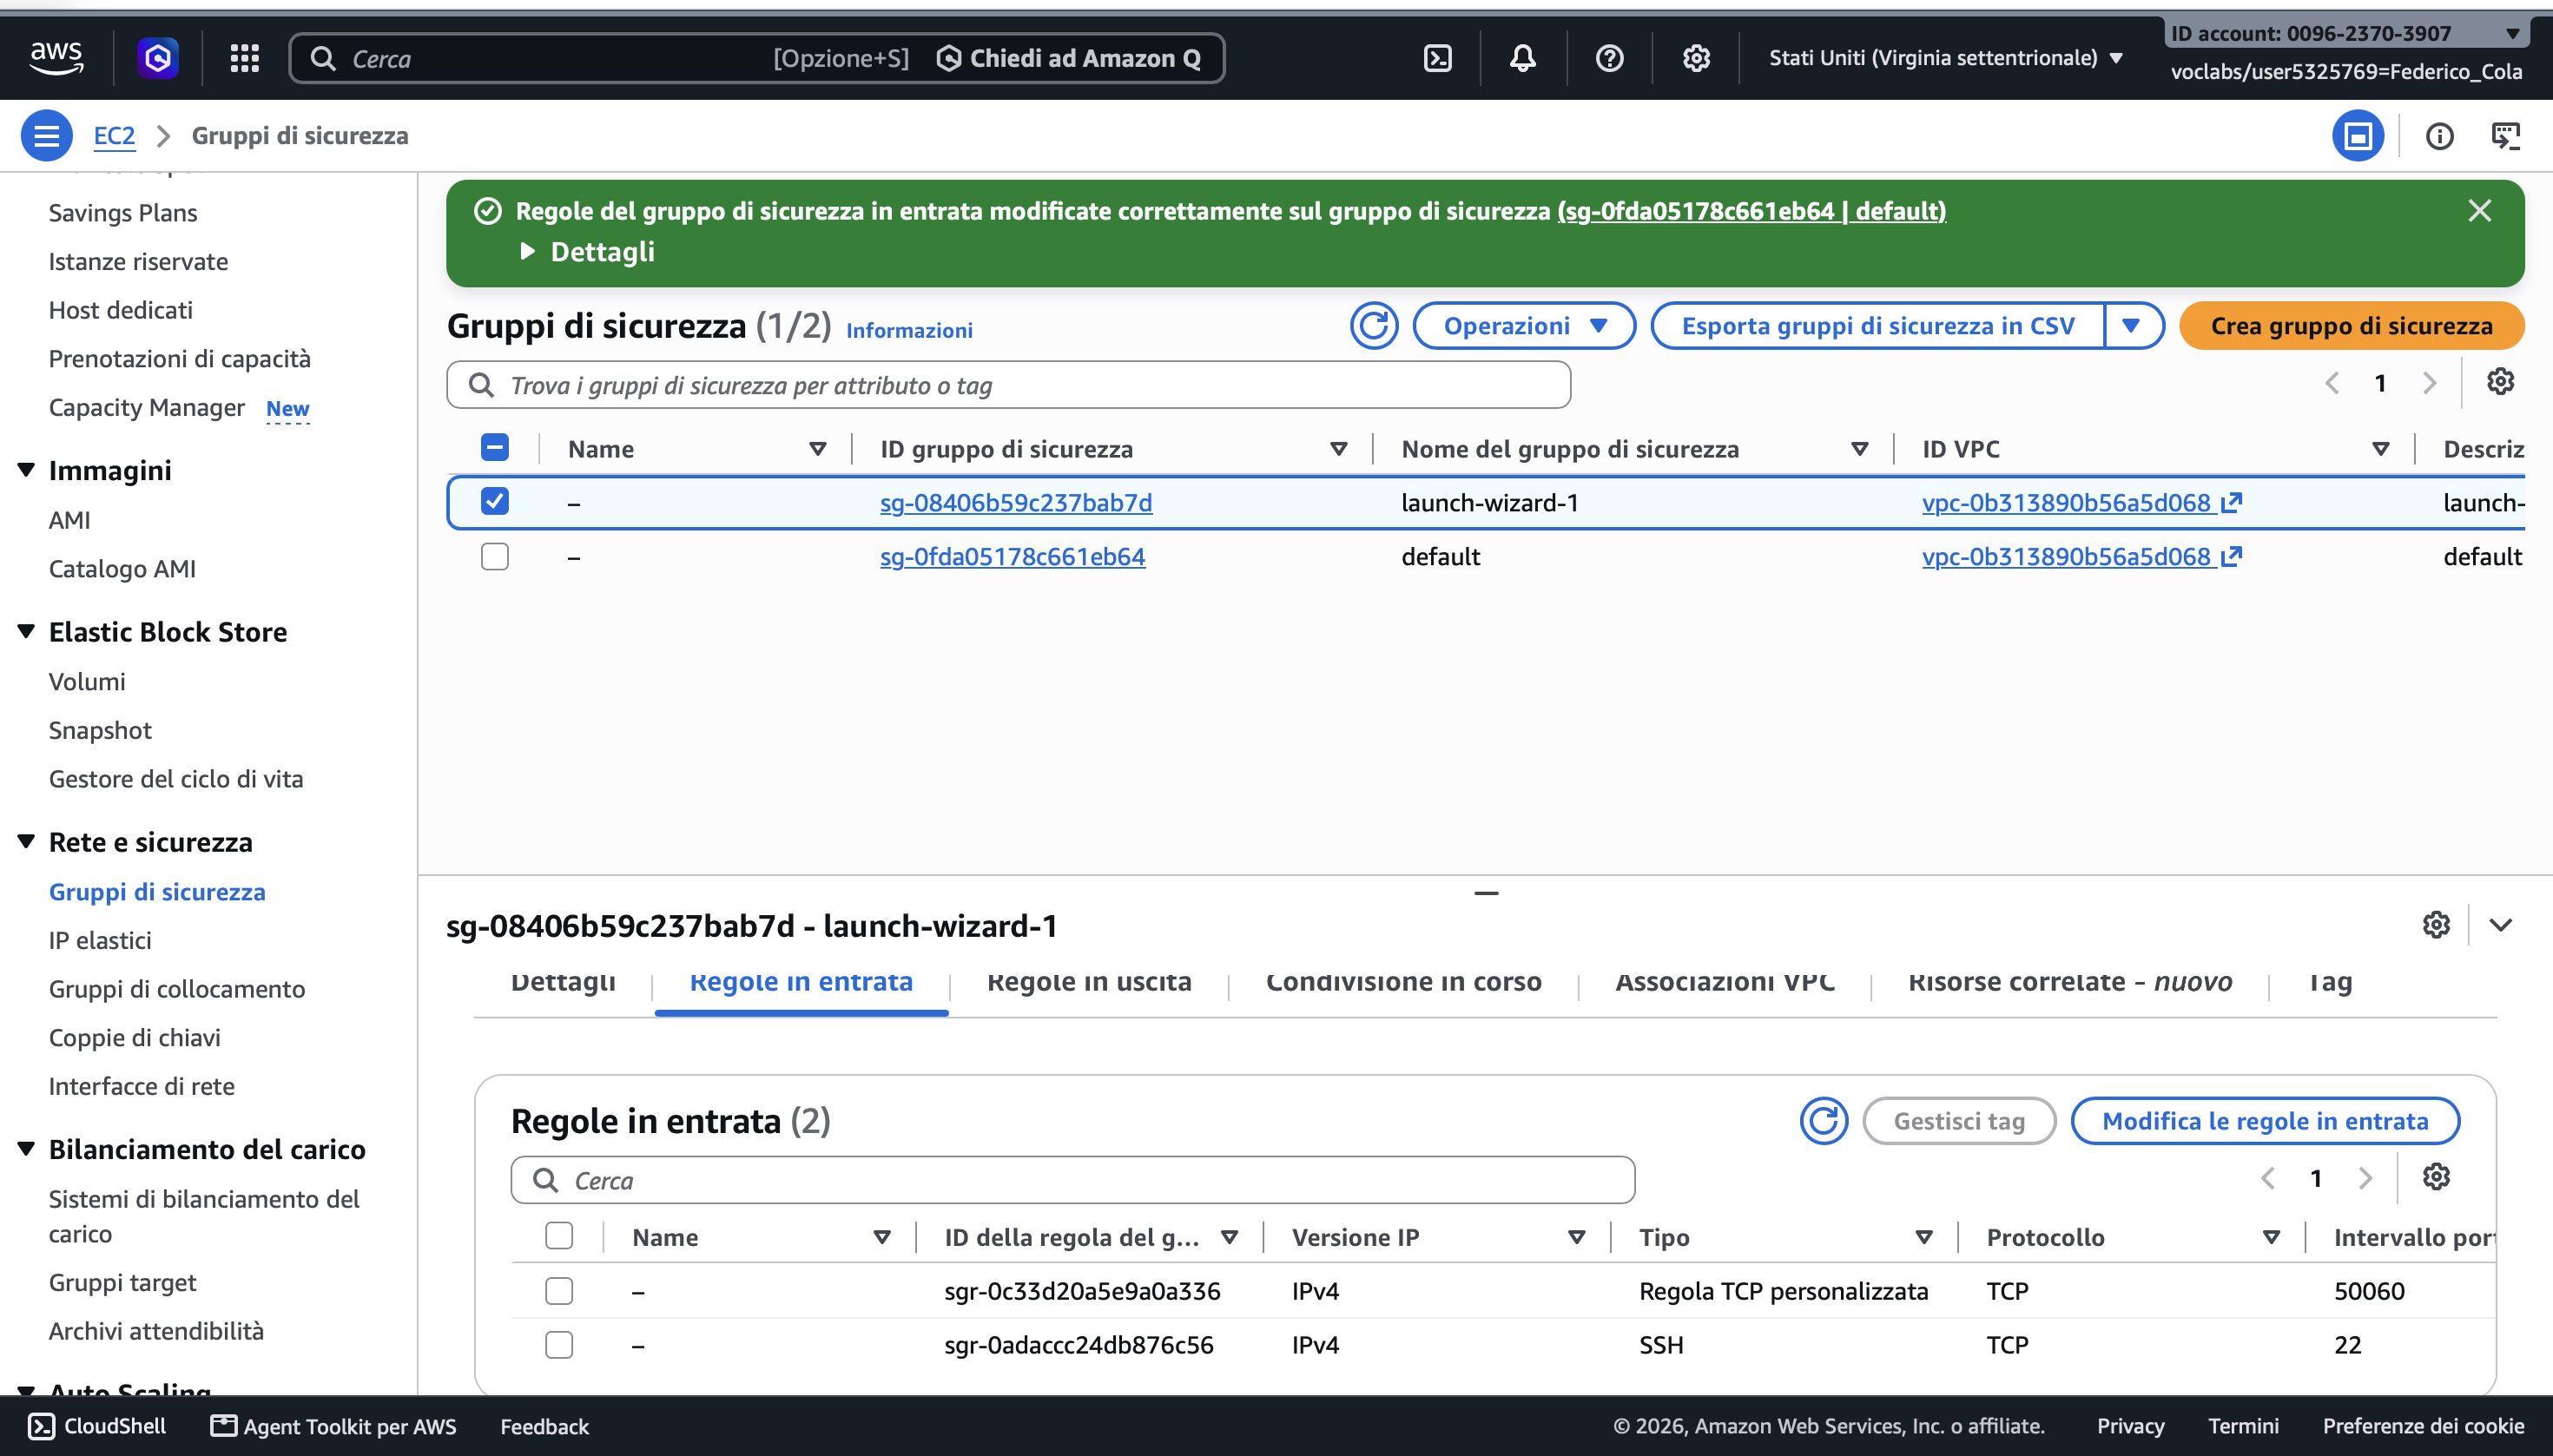
\includegraphics[width=\textwidth]{security-group.png}
\end{minipage}
\caption{Evidenza del deployment su istanza AWS EC2 reale: build e avvio
dei 5 container via Session Manager, con elezione del leader nei log
(sopra); stato dell'istanza con IP pubblico (in basso a sinistra); regola
del Security Group che apre la porta 50060 del proxy (in basso a destra).}
\label{fig:ec2-evidence}
\end{figure*}

\subsection{Limitazione nota: nessun cambio di membership dinamico}

La lista dei peer di ogni nodo è statica, letta una volta sola dal file
YAML all'avvio, e non cambia mai durante l'esecuzione: non esiste nessuna
RPC per aggiungere un nodo a un cluster già in funzione. Un nodo
\emph{già noto} che crasha e riparte si riallinea automaticamente (il
meccanismo di coerenza del log descritto sopra lo riporta in sincrono col
Leader), ma un nodo \emph{nuovo}, mai presente nella configurazione
iniziale, non può unirsi a runtime: nessun Leader lo conterebbe per il
quorum di maggioranza, e la Service Discovery non può scoprire un nodo che
nessun altro nodo conosce già. È il cambio di membership dinamico che il
paper di Raft tratta a parte (\S6, joint consensus) — deliberatamente
fuori scope per questo progetto, non richiesto dalla traccia.


\section{Results}
\label{sec:results}

Entrambi gli esperimenti sono stati eseguiti su un'istanza AWS EC2
(\texttt{t2.micro}) dell'infrastruttura di deployment, non sul portatile
di sviluppo: un primo tentativo in locale aveva prodotto misure rumorose e
non monotone (Sezione~\ref{sec:discussion}), e ripetere gli stessi
esperimenti su un'istanza dedicata — pur con hardware oggettivamente più
debole — ha dato un segnale molto più pulito, perché quella macchina non
esegue nient'altro in concorrenza con l'esperimento.

\subsection{Scalabilità: latenza RPC al variare di N}

Lo strumento \texttt{bench-client} misura la latenza di \texttt{Put} e
\texttt{Get} in sequenza (una RPC alla volta) contro il proxy, per N =
3, 5, 9, 20 nodi consensus. Ogni misura aggrega 5 ripetizioni indipendenti
da 50 operazioni ciascuna, dopo 5 operazioni di riscaldamento scartate per
stabilizzare le connessioni gRPC. La Tabella~\ref{tab:scalability} riporta
media, mediana (p50) e 95\textsuperscript{o} percentile (p95) in
millisecondi.

\begin{table}[H]
\centering
\caption{Latenza RPC (ms) al variare del numero di nodi N}
\label{tab:scalability}
\begin{tabular}{@{}lrrrrrr@{}}
\toprule
 & \multicolumn{3}{c}{PUT} & \multicolumn{3}{c}{GET} \\
\cmidrule(lr){2-4} \cmidrule(lr){5-7}
N & media & p50 & p95 & media & p50 & p95 \\
\midrule
3  & 9.35  & 9.10  & 10.48 & 3.00 & 2.92 & 3.62 \\
5  & 9.20  & 9.08  & 10.26 & 3.28 & 3.01 & 4.75 \\
9  & 9.31  & 8.86  & 13.46 & 3.09 & 2.87 & 4.14 \\
20 & 15.16 & 14.57 & 20.18 & 3.21 & 2.87 & 5.48 \\
\bottomrule
\end{tabular}
\end{table}

Il \texttt{GET} — una lettura locale sul Leader, teoricamente indipendente
da N perché non coinvolge replicazione — resta piatto attorno ai 3ms su
tutti i valori di N testati, esattamente come previsto dalla teoria. Il
\texttt{PUT} resta piatto (circa 9.2--9.35ms) da N=3 a N=9, per poi salire
nettamente a 15.16ms a N=20: coerente con Raft, dove il Leader deve
attendere l'ack della maggioranza (11 su 20 follower a N=20) prima di
poter committare, e la coda per l'ack più lento del gruppo di maggioranza
cresce con il numero di follower.

\subsection{Fault-tolerance: crash del leader}

Lo strumento \texttt{experiments/fault-tolerance} avvia un cluster di 5
nodi, ne scopre il Leader corrente via la RPC \texttt{GetStatus}, lo
uccide con \texttt{kill -9} per simulare un crash reale, e misura — via
timestamp a precisione di microsecondo nei log dei nodi superstiti — due
tempi: il tempo di \emph{rielezione} (dal crash alla prima
autoproclamazione di un nuovo Leader per un term successivo) e il tempo di
\emph{convergenza} (dal crash al momento in cui l'ultimo nodo superstite
riconosce quel nuovo Leader), su 10 trial indipendenti (Tabella~\ref{tab:fault-tolerance}).

\begin{table}[H]
\centering
\caption{Tempo di rielezione e convergenza dopo il crash del leader (ms, N=5, 10 trial)}
\label{tab:fault-tolerance}
\begin{tabular}{@{}lrrrrr@{}}
\toprule
 & media & p50 & p95 & min & max \\
\midrule
Rielezione  & 192.7 & 183.7 & 224.1 & 153.7 & 258.1 \\
Convergenza & 244.0 & 235.0 & 275.8 & 205.5 & 309.1 \\
\bottomrule
\end{tabular}
\end{table}

Entrambi i tempi cadono dentro, o appena sopra, l'intervallo di election
timeout configurato (150--300ms), come atteso. Il gap pressoché costante
di circa 50ms tra rielezione e convergenza corrisponde esattamente
all'heartbeat interval configurato: il nuovo Leader manda il proprio primo
\texttt{AppendEntries} subito dopo essersi eletto, e i follower lo
riconoscono quasi immediatamente. In tutti i 10 trial la convergenza è
stata completa (i superstiti hanno tutti riconosciuto il nuovo Leader) e
il servizio è sempre tornato operativo dopo il crash, verificato con una
scrittura riuscita via proxy subito dopo la stabilizzazione del nuovo
Leader.

\section{Discussion}
\label{sec:discussion}

\subsection{Interpretazione dei risultati sperimentali}

I due esperimenti confermano, con dati, il comportamento atteso
dell'algoritmo: il \texttt{GET} piatto su tutti
gli N testati conferma che una lettura locale sul Leader è davvero
indipendente dal numero di follower; il \texttt{PUT} piatto fino a N=9 e
in salita a N=20 conferma che il costo della replica si manifesta solo
quando il quorum di maggioranza diventa abbastanza numeroso da rendere
statisticamente rilevante l'attesa dell'ack più lento. I tempi di
rielezione e convergenza dell'esperimento di fault-tolerance cadono
esattamente dentro l'intervallo di election timeout configurato, e il
gap tra i due corrisponde all'heartbeat interval — nessuno dei due
esperimenti ha richiesto di rivedere ipotesi sul funzionamento del
sistema ed un suo successivo aggiornamento.

\textbf{Una lezione metodologica più ampia}, emersa nel percorso verso
questi dati: la prima misura di scalabilità, fatta sul portatile di
sviluppo, produceva numeri rumorosi e non monotoni — al punto che persino
il \texttt{GET}, che teoricamente non dovrebbe dipendere da N, mostrava le
stesse oscillazioni del \texttt{PUT}. Questo è stato il segnale che il
rumore di sistema (il portatile condiviso con l'ambiente di sviluppo
stesso) dominava sull'effetto reale. Ripetere l'esperimento su un'istanza
dedicata, pur con hardware più debole, ha eliminato quel rumore: la
dedizione dell'ambiente di misura conta più della sua potenza di calcolo
grezza.

\subsection{La regola di sicurezza \S5.4.2 osservata dal vivo}

Durante il deployment su AWS EC2 (non durante gli esperimenti controllati
di questa sezione, ma nel corso della verifica del sistema in un ambiente
reale), un riavvio dell'istanza ha offerto una conferma pratica della
regola discussa in Sezione~\ref{sec:background}: una \texttt{Get} su una
chiave scritta prima dello stop ha restituito \texttt{found=false}, non
per perdita di dati ma perché \texttt{commitIndex} e \texttt{lastApplied}
sono volatili e si azzerano a ogni riavvio (Sezione~\ref{sec:details}). Il
nuovo Leader, eletto in un nuovo term, non ha potuto far avanzare il
proprio \texttt{commitIndex} oltre le entry di un term precedente finché
non è avvenuta una nuova scrittura nel term corrente — a quel punto,
\texttt{commitIndex} è avanzato in ordine di log oltre entrambe le entry
in un colpo solo, e la vecchia chiave è ridiventata immediatamente
visibile. Un episodio degno di nota che ha costituito una verifica del processo logico più sottile dell'algoritmo.

\subsection{Limiti noti}

Due scelte di scope, già motivate in Sezione~\ref{sec:details}, restano
limiti espliciti del sistema così com'è: (1) nessun cambio di membership
dinamico — un nodo può rientrare nel cluster dopo un crash, ma un nodo mai
presente nella configurazione iniziale non può unirsi a runtime; (2)
nessuna compattazione del log \emph{sui consensus node stessi} — il
servizio Snapshot \& backup compatta correttamente lo storico in
checkpoint esterni, ma non tronca il log persistito di ogni nodo, che
quindi cresce indefinitamente con l'uso prolungato del sistema.

\section{Conclusions}
\label{sec:conclusions}

Questo lavoro ha realizzato un key-value store distribuito, replicato e
fortemente consistente, con un'implementazione di Raft costruita da zero
(elezione del leader, replicazione del log, e le regole di sicurezza che
governano l'avanzamento del commit) e verificata sia con unit test sia con
processi reali comunicanti in rete. Tutti i requisiti architetturali della
traccia sono soddisfatti: i tre tipi di nodo (consensus, client proxy,
snapshot \& backup), la comunicazione interamente su gRPC/Protocol
Buffers, i due pattern architetturali richiesti (Service Discovery e
Circuit Breaker), e un deployment containerizzato con Docker Compose
verificato su una vera istanza AWS EC2, raggiungibile e funzionante
dall'esterno.

I due esperimenti di valutazione richiesti — scalabilità e
fault-tolerance — hanno prodotto dati puliti e coerenti con la teoria di
Raft: latenza di lettura indipendente dal numero di nodi, latenza di
scrittura che cresce solo quando il quorum di maggioranza diventa
numeroso, e tempi di rielezione/convergenza dopo un crash del leader in
linea con i parametri di timeout configurati. Il percorso verso questi
risultati ha anche prodotto una lezione metodologica di per sé utile:
misurare la latenza di un sistema distribuito richiede un ambiente di
misura dedicato, non necessariamente potente.

Il sistema ha due limiti dichiarati, entrambi scelte di scope deliberate e
non richieste dalla traccia: l'assenza di un meccanismo di cambio di
membership dinamico (un nodo può ripresentarsi dopo un crash, ma non può
unirsi ex novo a un cluster già in funzione), e l'assenza di compattazione
del log \emph{sui consensus node stessi} (il servizio Snapshot \& backup
compatta correttamente lo storico in checkpoint esterni, ma il log
persistito di ogni nodo cresce indefinitamente). Entrambi rappresentano
estensioni naturali per un lavoro futuro, così come l'esplorazione di
cluster di dimensioni ancora maggiori per caratterizzare più a fondo la
curva di scalabilità osservata tra N=9 e N=20.

\bibliographystyle{IEEEtran}
\bibliography{references}
% TODO: creare references.bib — almeno il paper originale di Raft
% (Ongaro & Ousterhout, "In Search of an Understandable Consensus
% Algorithm") e la documentazione gRPC/Protobuf se citata.

\end{document}